\begin{frame}{$\phi$-FEM Method}
	\textbf{Main ideas :} \hspace{30pt} \refappendix{frame:phifem}  \small
	
	\begin{minipage}[t]{0.48\linewidth}
		\begin{itemize}[\textbullet]
			\item Domain defined by a LevelSet Function $\phi$.
		\end{itemize}
		\centering
		\pgfimage[width=0.6\linewidth]{images/hybrid/PhiFEM_level_set.png}
	\end{minipage} \hfill
	\begin{minipage}[t]{0.48\linewidth}
		\begin{itemize}[\textbullet]
			\item We are looking for $w$ such that $u=\phi w+g$. \\
			Thus, the decoder is written as
			\begin{equation*}
				u_\theta(x)=\mathcal{D}_{\theta_w}(x) = \phi(x)\sum_{i=1}^{N}(\theta_w)_i\varphi_i+g(x)
			\end{equation*}
		\end{itemize}
	\end{minipage}

	\begin{itemize}[\textbullet]
		\item Mesh of a fictitious domain containing $\Omega$.
	\end{itemize}
	\begin{center}
		\begin{minipage}{0.43\linewidth}
			\centering
			\pgfimage[width=\linewidth]{images/more/PhiFEM_domain.png}
		\end{minipage} \hfill
		\begin{minipage}{0.1\linewidth}
			\centering
			\pgfimage[width=\linewidth]{images/more/PhiFEM_fleche.png} 
		\end{minipage} \hfill
		\begin{minipage}{0.43\linewidth}
			\centering
			\pgfimage[width=\linewidth]{images/more/PhiFEM_domain_considered.png}
		\end{minipage}
	\end{center}
\end{frame}

\begin{frame}{Impose exact BC in PINNs}
	Considering the least squares form of our PDE, we impose the exact boundary conditions by writing our solution as
	\begin{equation*}
		u_\theta=\phi w_\theta + g
	\end{equation*}
	where $w_\theta$ is our decoder (defined by a neural network such as an MLP).
	
	We then consider the same minimization problem by removing the cost function associated with the boundary
	\begin{equation*}
		\theta_u=\arg\min_{\theta\in\mathbb{R}^N} J_{in}(\theta)+\Ccancel[red]{J_{bc}(\theta)}
	\end{equation*}
	with 
	\begin{equation*}
		J_{in}(\theta)=\frac{1}{2}\int_\Omega (L(\phi w_\theta + g) - f)^2  \qquad \text{and} \qquad \Ccancel[red]{J_{bc}(\theta)=\frac{1}{2}\int_{\partial\Omega} (v_\theta-g)^2}
	\end{equation*}	
%	\vspace{-20pt}
%	\begin{figure}[htb]
%		\hspace{-105pt}
%		\begin{tikzpicture}
%			\draw[->, blue, line width=1pt] (0,1) -- (0.15,0.3);
%		\end{tikzpicture} 
%	\end{figure}
%	\begin{equation*}
%		J_{in}(\theta)=\frac{1}{2}\int_\Omega (L(\phi w_\theta + g) - f)^2
%	\end{equation*}	
\end{frame}

\begin{frame}{Correct PINNs prediction with $\phi$FEM}
	\vspace{-20pt}
	\begin{figure}[htb]
		\centering
		\resizebox{\textwidth}{!}{%
			\begin{tikzpicture}
				\node at (0,0.8) {1 Geometry - 1 Function};
				\node[draw=none, inner sep=0pt] at (0,0) {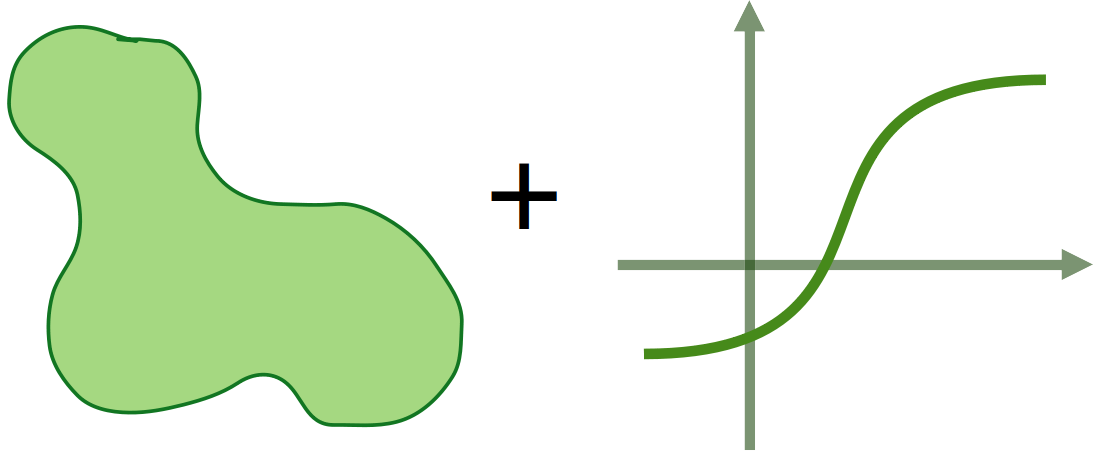
\includegraphics[width=2cm]{images/hybrid/objective_onegeom_onefct.png}};
				\node at (0,-1) {$\begin{aligned}[t]
						\; \phi \quad \text{\small and} \quad &f \\
						\; (\text{\small and} \quad &g)
					\end{aligned}$};
				
				\draw[->, title, line width=1.5pt] (2,0.1) -- (3,0.1);
				
				\node[align=center] at (4,1) {Get PINNs \\ prediction};
				\node[draw=none, inner sep=0pt] at (4,-0.1) {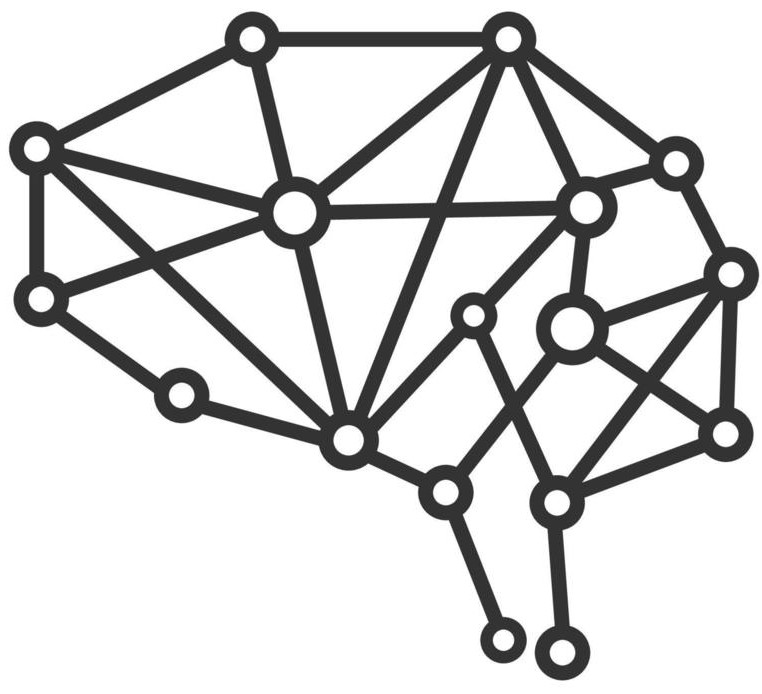
\includegraphics[width=1.5cm]{images/hybrid/objective_pinns.jpg}};
				\node at (4,-1) {$u_{NN}=\phi w_{NN}+g$};
				
				% Ajouter une flèche entre les deux rectangles
				\draw[->, title, line width=1.5pt] (5,0.1) -- (6,0.1);
				
				\node[align=center] at (7.8,1) {Correct prediction \\ with $\phi$-FEM};
				\node[draw=none, inner sep=0pt] at (7.8,-0.1) {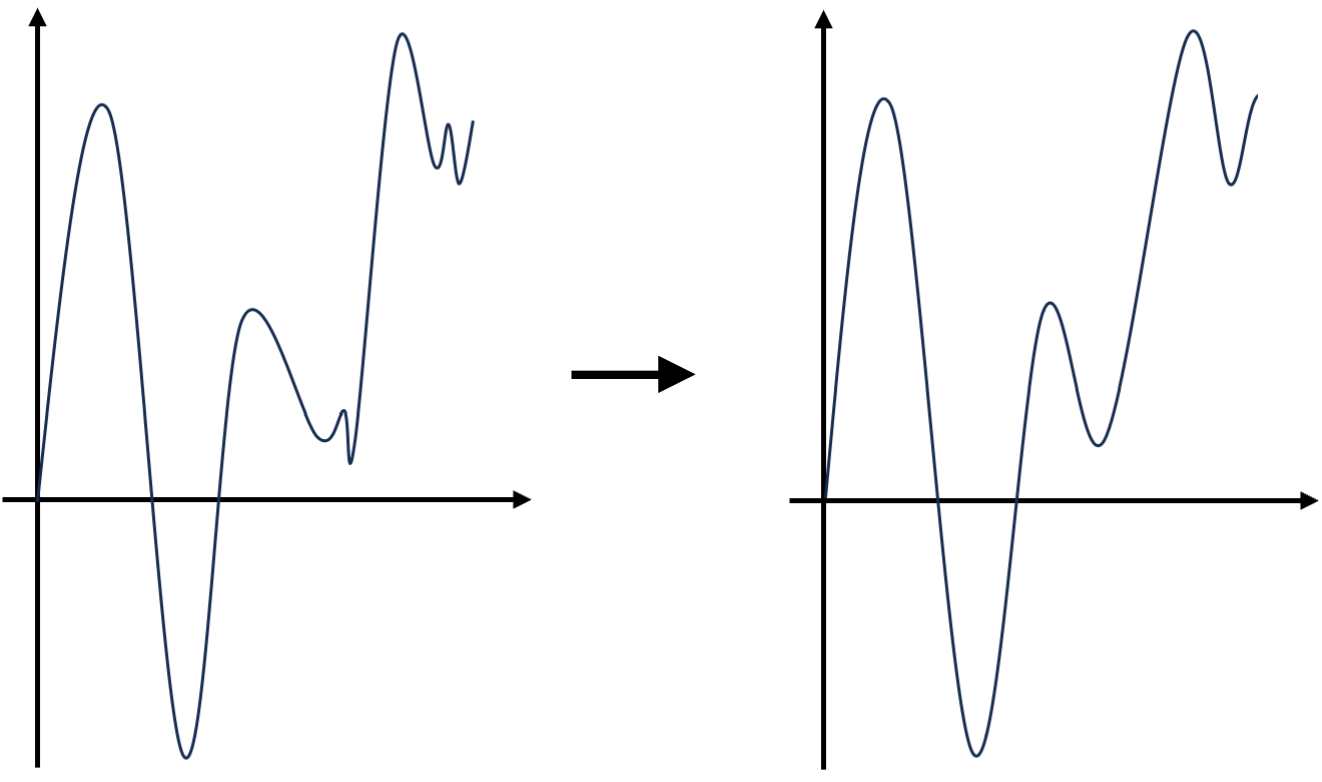
\includegraphics[width=2.5cm]{images/hybrid/objective_corr.png}};		
				\node at (7.8,-1) {$u_{NN}\rightarrow\tilde{u}=u_{NN}+\phi C$};
			\end{tikzpicture} 
		}%
	\end{figure}

	\vspace{-10pt}

	\textbf{Correct by adding :} Considering $u_{NN}$ as the prediction of our PINNs (trained to learn the solution of the elliptic problem), the correction problem consists in writing the solution as
	\begin{equation*}
		\tilde{u}=u_{NN}+\underset{\textcolor{blue}{\approx 0}}{\fcolorbox{blue}{white}{$\tilde{C}$}}
	\end{equation*}

	\vspace{-8pt}
	\begin{minipage}{\linewidth}
		\setstretch{0.5}
		and searching $\tilde{C}: \Omega \rightarrow \mathbb{R}^d$ such that
		\begin{equation*}
			\left\{\begin{aligned}
				L(\tilde{C})&=\tilde{f}, \; &&\text{in } \Omega, \\
				\tilde{C}&=0, \; &&\text{on } \Gamma,
			\end{aligned}\right. %\tag{$\mathcal{C}_{+}$} %\label{corr_add}
		\end{equation*}
		with $\tilde{f}=f-L(u_{NN})$ and $\tilde{C}=\phi C$ for the $\phi$-FEM method.
	\end{minipage}
\end{frame}